\documentclass[11pt,a4paper]{article}
\usepackage[a4paper,left=2.1cm,right=2.1cm,top=2cm,bottom=2.2cm]{geometry}
\usepackage{newtxtext,newtxmath,graphicx,booktabs,array,float,microtype,xcolor,hyperref}
\usepackage{setspace}
\usepackage{xurl}
\usepackage{caption}
\setstretch{1.1}
\hypersetup{colorlinks=true,urlcolor=blue!50!black,linkcolor=black}
\renewcommand{\arraystretch}{1.13}
\newcommand{\mac}{\mathrm{MAC}}
\begin{document}
\begin{titlepage}
\centering
\vspace*{0.45cm}

\includegraphics[width=6.0cm]{../assets/uom_logo.png}
\par\vspace{1.9cm}
{\Large\bfseries EN3150 Assignment 03\par}
\vspace{0.38cm}
{\LARGE\bfseries Resource-Constrained CNN for\par}
{\LARGE\bfseries Edge Image Classification\par}
\vspace{2.95cm}
{\Large\bfseries Project Team: Cybertron\par}
\vspace{1.1cm}
\begin{tabular}{@{}l@{\quad--\quad}l@{}}
230018T & Adikaram D.M.G.H.\\[3pt]
230074J & Bandara H.Y.W.\\[3pt]
230476T & Perera G.M.B.\\[3pt]
230486A & Perera U.I.H.
\end{tabular}
\vfill
{\large Department of Electronic and Telecommunication Engineering\par}
{\large University of Moratuwa\par}
\vspace{0.95cm}
{\large October 19, 2026\par}
\vspace{1.0cm}
\end{titlepage}
\pagestyle{plain}
\section{Introduction and dataset}
This assignment studies whether a small convolutional network can classify images using fewer memory and arithmetic resources. We compare a standard CNN (Model A) with an otherwise similar depthwise-separable CNN (Model B). We then compare optimizers and examine the size of two lightweight published networks.

\textbf{Dataset:} UCI Optical Recognition of Handwritten Digits via scikit-learn. This is the UCI Optical Recognition of Handwritten Digits data provided by scikit-learn: 1,797 images in ten categories (0 to 9). The original images are 8$\times$8 grayscale. Each image is enlarged by bilinear interpolation to 32$\times$32 and copied to three identical channels. Upscaling does not introduce new information. This makes the dataset appropriate for an offline, low-resolution proof of concept, but easier than actual field photographs.

\begin{table}[H]\centering
\caption{Dataset split. A stratified random split with seed 42 was used.}
\begin{tabular}{lrr}\toprule
Subset & Number of images & Percentage \\ \midrule
Training & 1257 & approximately 70\% \\
Validation & 270 & approximately 15\% \\
Testing & 270 & approximately 15\% \\
Total & 1797 & 100\% \\ \bottomrule
\end{tabular}\end{table}

All samples were shuffled and split with stratification before training, so the same input images were used for every model. Pixel intensities were normalized to [0,1]. The classes were: 0, 1, 2, 3, 4, 5, 6, 7, 8, 9. Testing images were kept separate from the optimizer selection process.

\section{Custom CNN architecture}
Both models use three convolution stages with ReLU, batch normalization, and $2\times2$ max pooling after each stage. The channel widths are 16, 32, and 64. We use global-average pooling rather than flattening the large feature maps; this keeps the dense layer small. The fully connected layers use 32 hidden units and 10 output logits. We used cross-entropy loss.

\begin{table}[H]\centering\small
\caption{Network design and trainable parameters per layer. Input is $32\times32\times3$.}
\begin{tabular}{p{5.1cm}rrp{4cm}}\toprule
Layer & Model A & Model B & Output size \\ \midrule
Conv1: $3\times3$, $3\rightarrow16$ & 448 & 91 & $32\times32\times16$ \\
BatchNorm1 & 32 & 32 & same \\
MaxPool1: $2\times2$ & 0 & 0 & $16\times16\times16$ \\
Conv2: $3\times3$, $16\rightarrow32$ & 4,640 & 688 & $16\times16\times32$ \\
BatchNorm2 & 64 & 64 & same \\
MaxPool2: $2\times2$ & 0 & 0 & $8\times8\times32$ \\
Conv3: $3\times3$, $32\rightarrow64$ & 18,496 & 2,400 & $8\times8\times64$ \\
BatchNorm3 & 128 & 128 & same \\
MaxPool3: $2\times2$ & 0 & 0 & $4\times4\times64$ \\
Global average pooling & 0 & 0 & 64 \\
Dense 64$\rightarrow$32 & 2,080 & 2,080 & 32 \\
Dense 32$\rightarrow$10 & 330 & 330 & 10 \\
\midrule
\textbf{Total} & \textbf{26,218} & \textbf{5,813} & \\ \bottomrule
\end{tabular}\end{table}

For an ordinary convolution, the parameter count is $k^2C_{\mathrm{in}}C_{\mathrm{out}}+C_{\mathrm{out}}$, including bias. For depthwise separable convolution we use a depthwise kernel without bias followed by a biased $1\times1$ pointwise layer: $k^2C_{\mathrm{in}}+C_{\mathrm{in}}C_{\mathrm{out}}+C_{\mathrm{out}}$. Thus the first stage uses $3^2(3)+(3)(16)+16=91$ parameters rather than $(3^2(3)+1)16=448$. The final parameter counts are read from the actual PyTorch models.

ReLU computes $\max(0,x)$, avoiding an exponential at each hidden neuron; this is straightforward on small processors. Pooling reduces spatial dimensions and computations, and the small dense head reduces stored weights. The models produce logits; softmax is not necessary to decide which class has the largest score.

\section{Training and optimizer comparison}
We trained both custom models for 25 epochs, using batch size 64 and random seed 42. Model A and Model B use Adam ($\eta=0.001$). We also trained Model B using SGD ($\eta=0.02$) and SGD with momentum $0.9$ (same learning rate). Learning rates were chosen as simple starting values, not from an exhaustive search. The network with lowest \emph{validation loss} during training was selected before running the test evaluation. This prevents an unstable final epoch from deciding the result.

\begin{table}[H]\centering\small
\caption{Optimizer comparison on Model B (macro-average precision/recall).}
\begin{tabular}{lrrrrr}\toprule
Optimizer & Epochs & Best epoch & Test accuracy & Precision & Recall \\ \midrule
SGD & 25 & 25 & 53.7\% & 58.8\% & 53.3\% \\
SGD + momentum & 25 & 25 & 94.4\% & 94.9\% & 94.4\% \\
Adam & 25 & 23 & 95.9\% & 96.1\% & 95.9\% \\
\bottomrule\end{tabular}\end{table}

\begin{figure}[H]\centering
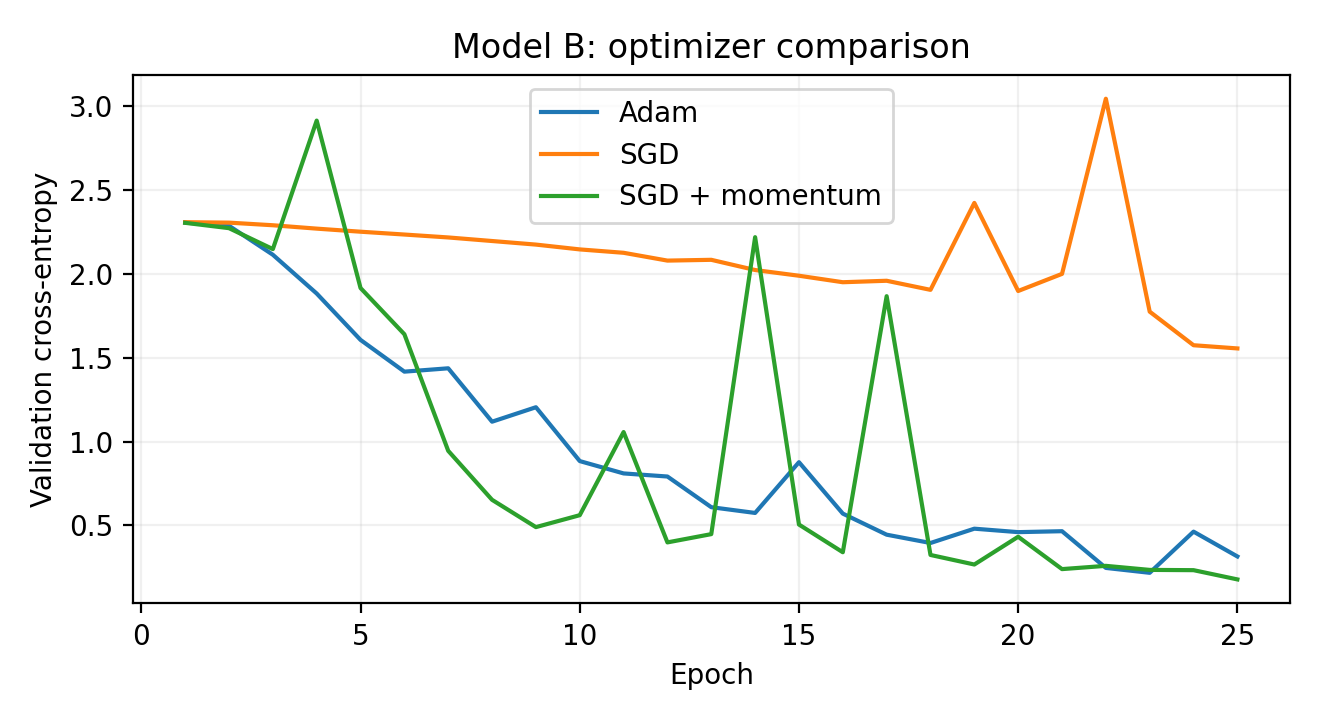
\includegraphics[width=0.80\linewidth]{../results/plots/optimizers_val_loss.png}
\caption{Measured validation loss for each optimizer. The curves illustrate differences in convergence speed; occasional spikes are also visible.}\end{figure}

Momentum accumulates a moving direction from recent gradients. It can reduce oscillation and help a small network converge more quickly. In these runs, SGD with momentum outperformed plain SGD; Adam reached the highest test accuracy of the three Model B optimizer trials. The values in Table 3 should be interpreted for this one seed and these particular settings.

\section{Custom CNN performance and cost}
\begin{table}[H]\centering\small
\caption{Real test performance and resource measurements. Time includes training and validation on CPU, averaged per epoch.}
\begin{tabular}{lrrrrr}\toprule
Model & Parameters & Saved KB & MACs/image & Seconds/epoch & Test accuracy \\ \midrule
Model A & 26,218 & 111.7 & 2,804,032 & 0.30 & 97.8\% \\
Model B & 5,813 & 33.2 & 396,608 & 0.28 & 95.9\% \\
\bottomrule\end{tabular}\end{table}

\begin{figure}[H]\centering
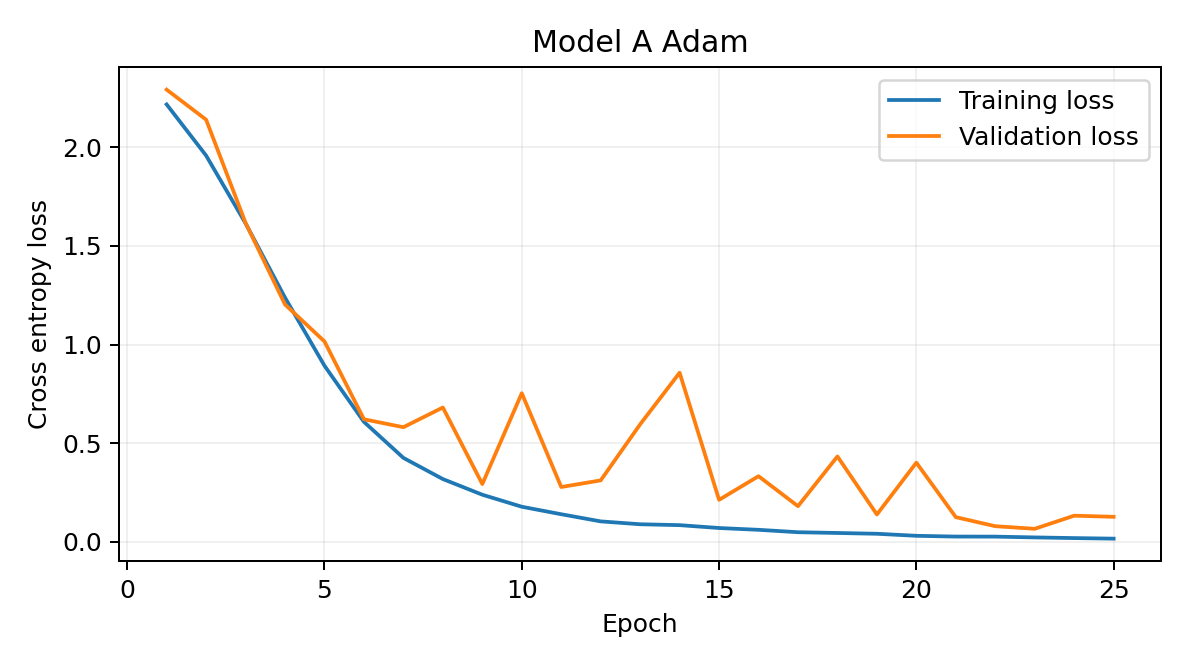
\includegraphics[width=0.48\linewidth]{../results/plots/model_a_adam_loss.png}
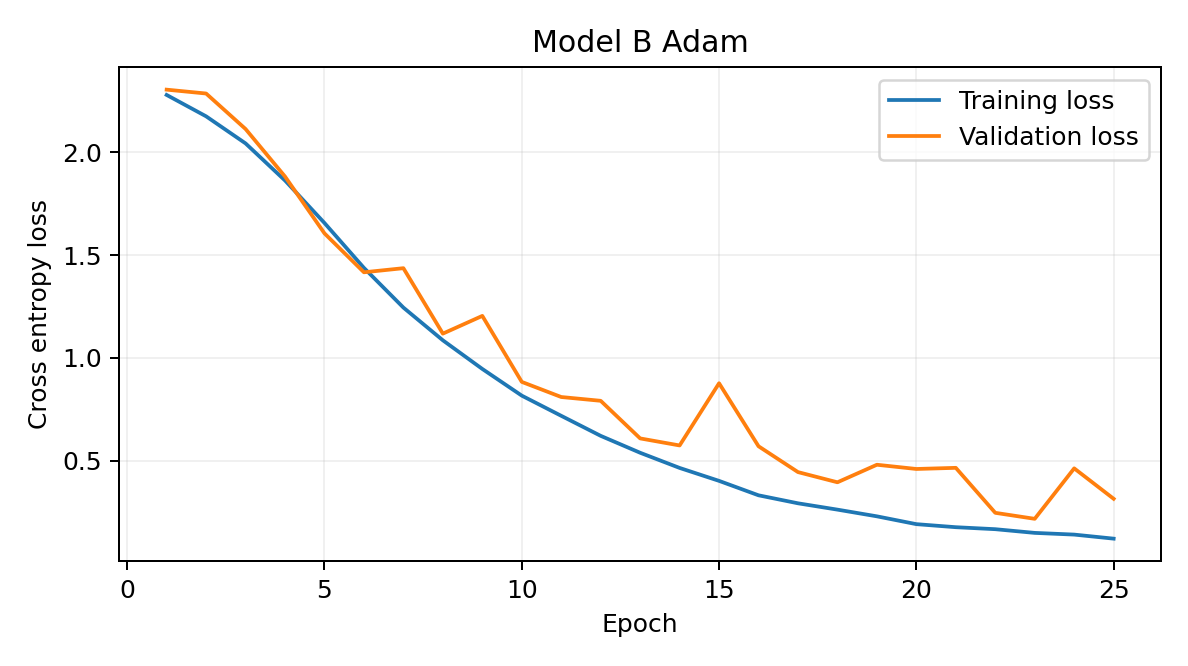
\includegraphics[width=0.48\linewidth]{../results/plots/model_b_adam_loss.png}
\caption{Training and validation cross-entropy over 25 epochs for Models A and B.}\end{figure}

\begin{figure}[H]\centering
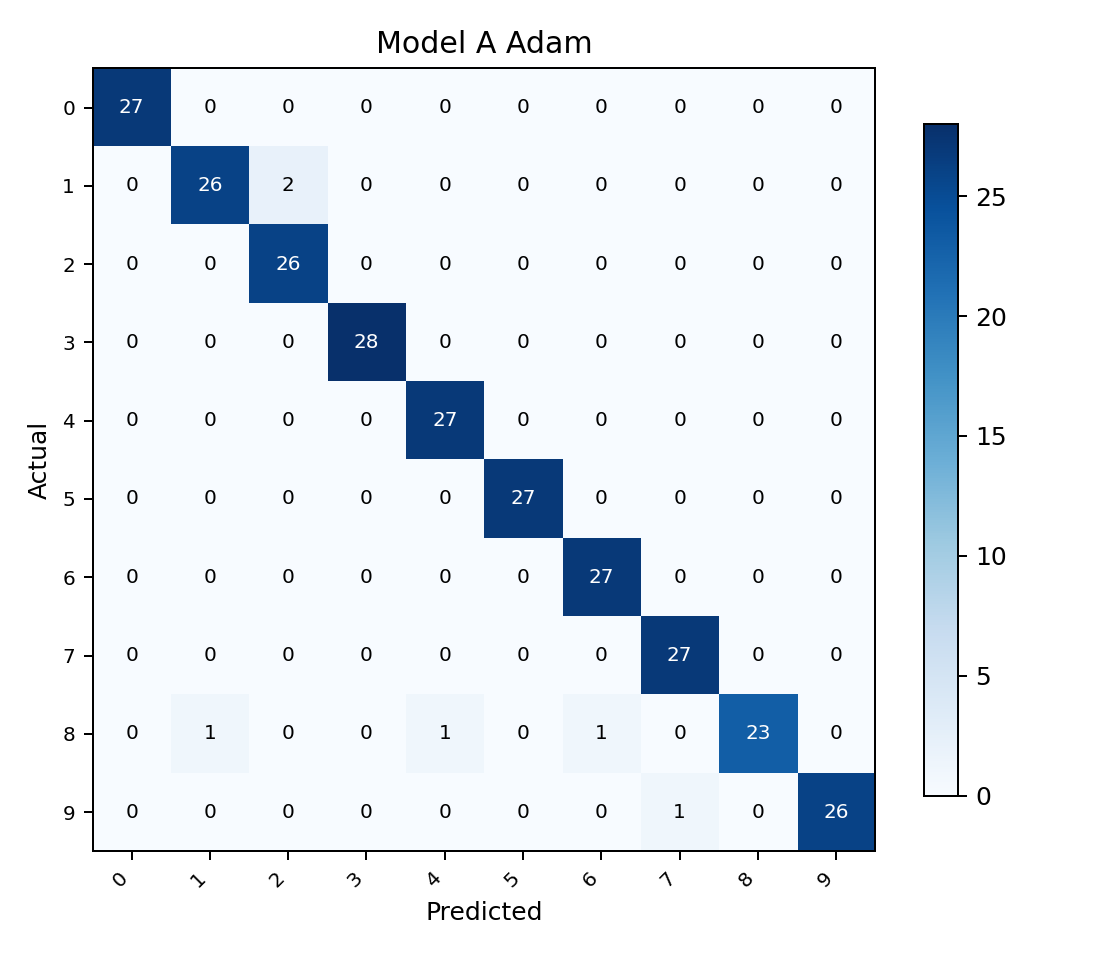
\includegraphics[width=0.47\linewidth]{../results/plots/model_a_adam_confusion.png}
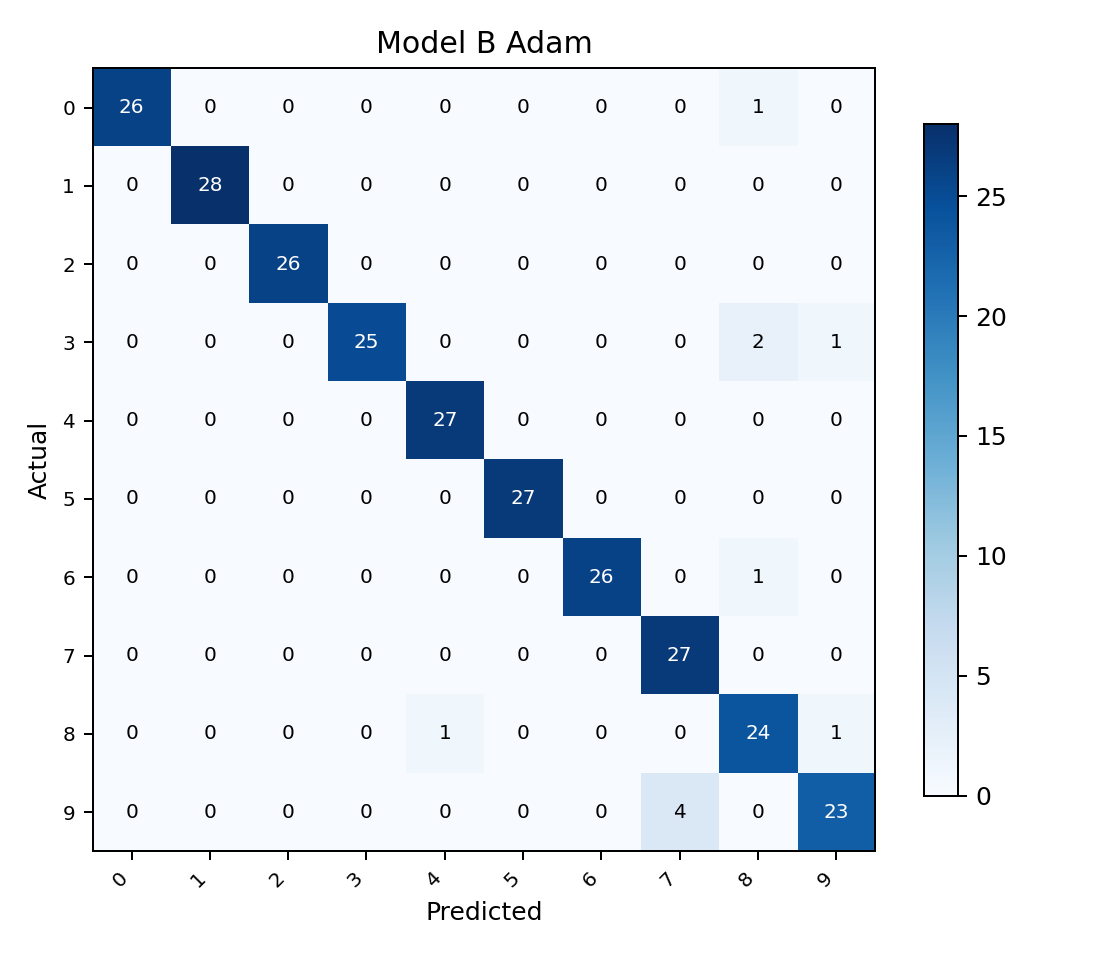
\includegraphics[width=0.47\linewidth]{../results/plots/model_b_adam_confusion.png}
\caption{Test-set confusion matrices for Models A (left) and B (right). Rows are actual classes; columns are predicted classes.}\end{figure}

Model B has 77.8\% fewer trainable parameters and 85.9\% fewer counted MACs, while its test accuracy is 95.9\% compared with 97.8\% for Model A. Both models have similar measured seconds per epoch on this particular CPU; very small workloads have Python/data-loading overhead, so arithmetic reductions need not produce proportional wall-clock speedups. Model A had a macro precision of 97.8\% and macro recall of 97.8\%; Model B had a macro precision of 96.1\% and macro recall of 95.9\%. Model B's actual saved PyTorch state file is larger than just four bytes times parameter count, because serialized files include batch-normalization buffers and metadata.

\section{Lightweight pretrained networks}
The comparison architectures are MobileNetV2 and SqueezeNet1.1, initialized with ImageNet pretrained weights from torchvision. For the same 10-class task, their measured results and sizes are:

\begin{table}[H]\centering\small
\caption{Pretrained-model comparison. Model sizes are actual PyTorch checkpoints; MACs are estimates for one 32$\times$32 image.}
\begin{tabular}{lrrrr}\toprule
Architecture & Parameters & Size (MB) & MACs/image & Test accuracy \\ \midrule
MobileNetV2 & 2,236,682 & 8.76 & 6,124,928 & 77.0\% \\
SqueezeNet1.1 & 727,626 & 2.79 & 2,995,904 & 26.7\% \\
\bottomrule\end{tabular}\end{table}

Both pretrained models were fine-tuned using the same deterministic split. Test accuracy, macro-averaged precision and recall were computed using the saved best-validation checkpoint.

\begin{table}[H]\centering\small
\caption{Pretrained-model evaluation on the 270 held-out digit images (macro averages).}
\begin{tabular}{lrrrr}\toprule
Model & Precision & Recall & Trained epochs & Best epoch \\ \midrule
MobileNetV2 & 81.2\% & 77.1\% & 10 & 10 \\
SqueezeNet1.1 & 22.5\% & 26.3\% & 10 & 10 \\
\bottomrule\end{tabular}\end{table}

\begin{figure}[H]\centering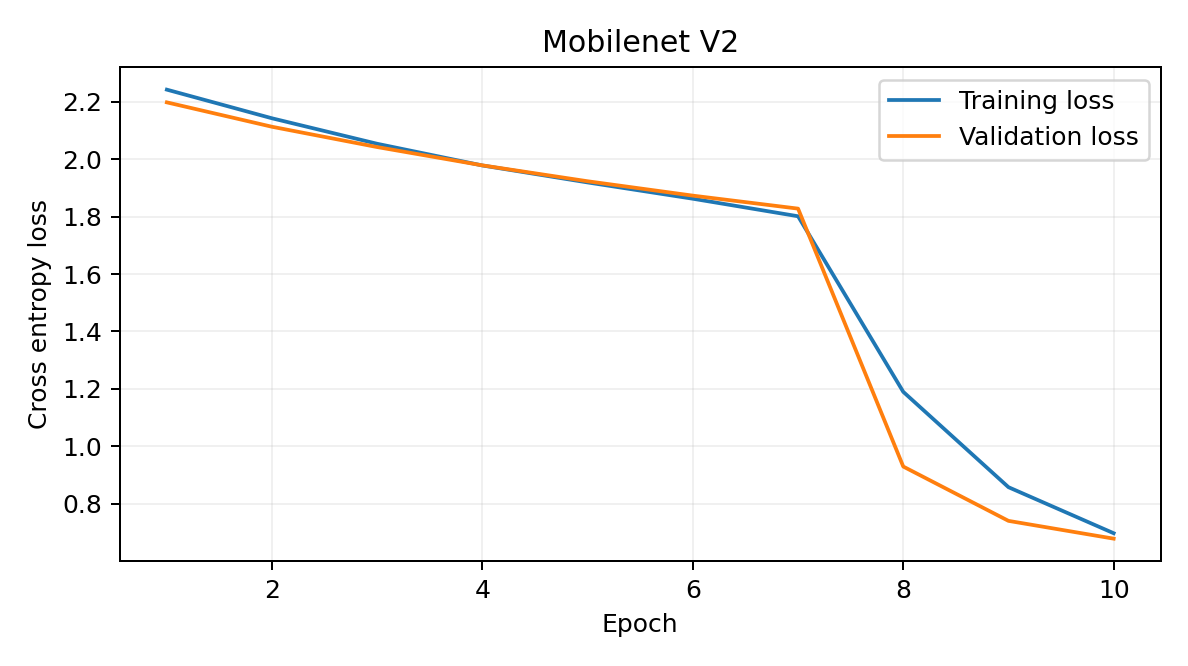
\includegraphics[width=0.46\linewidth]{../results/plots/mobilenet_v2_loss.png}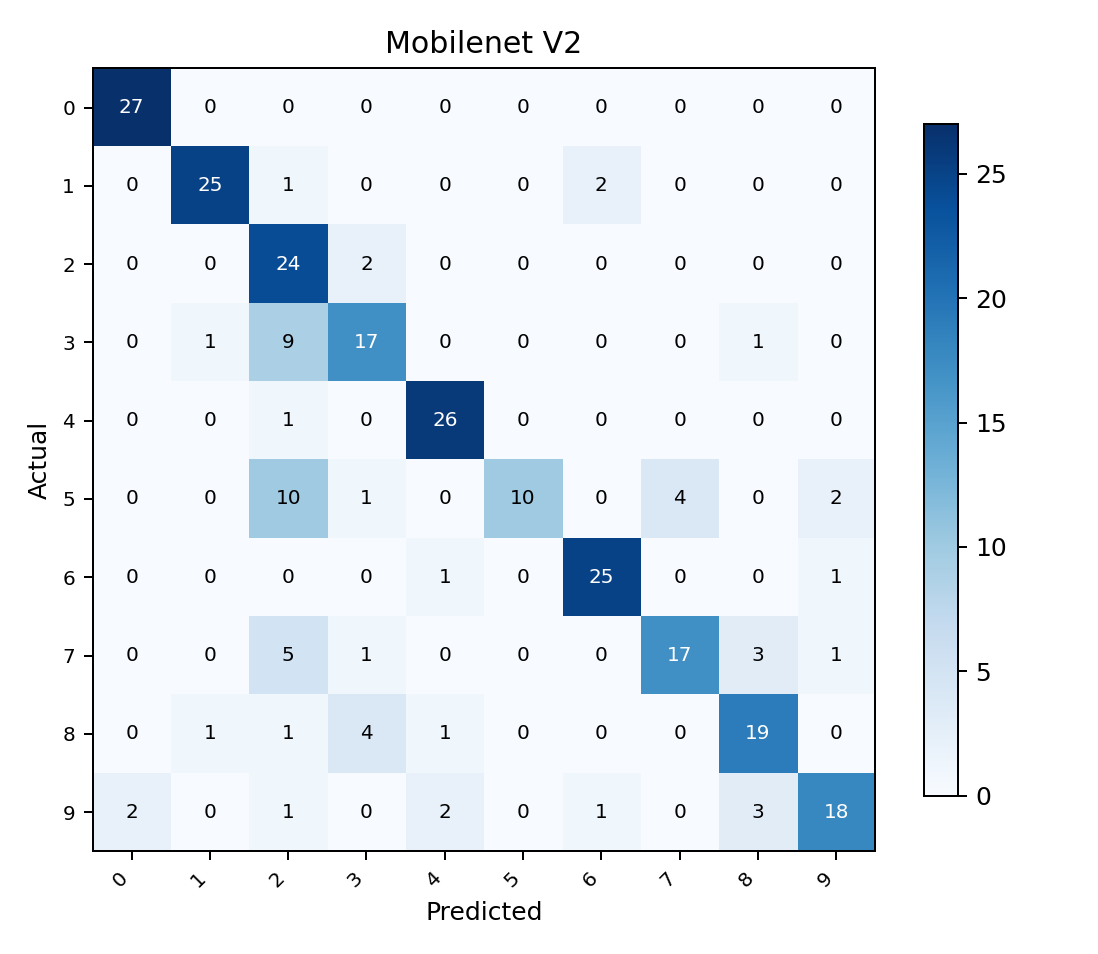
\includegraphics[width=0.46\linewidth]{../results/plots/mobilenet_v2_confusion.png}\caption{MobileNetV2 training and validation loss (left) and test confusion matrix (right).}\end{figure}
\begin{figure}[H]\centering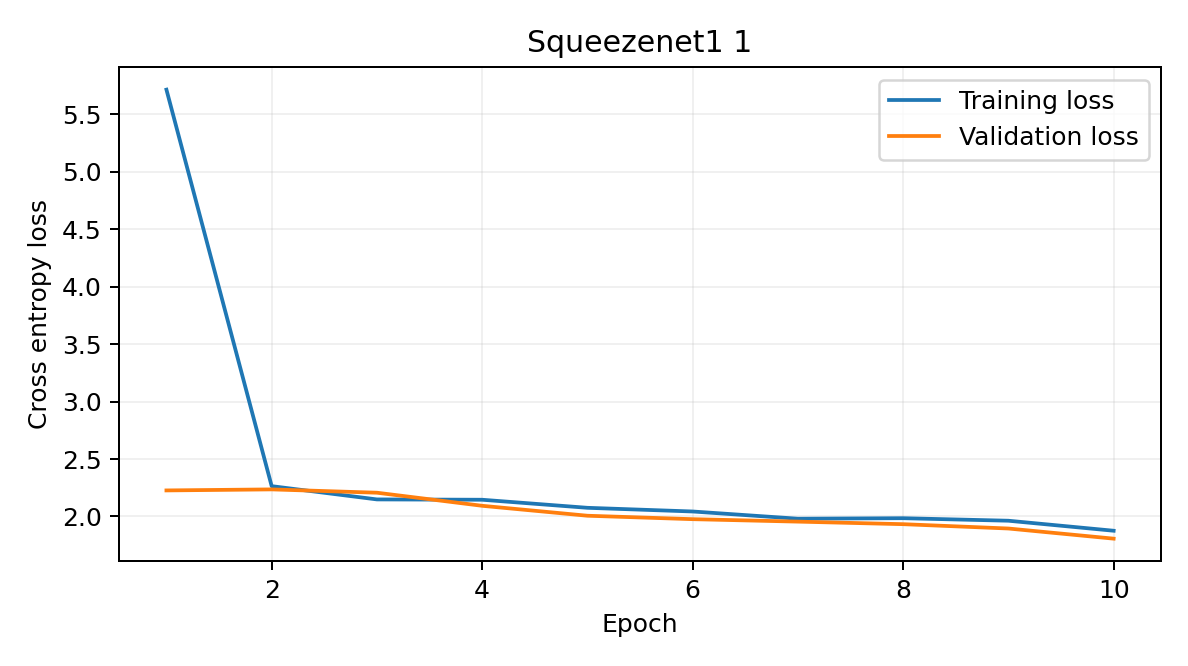
\includegraphics[width=0.46\linewidth]{../results/plots/squeezenet1_1_loss.png}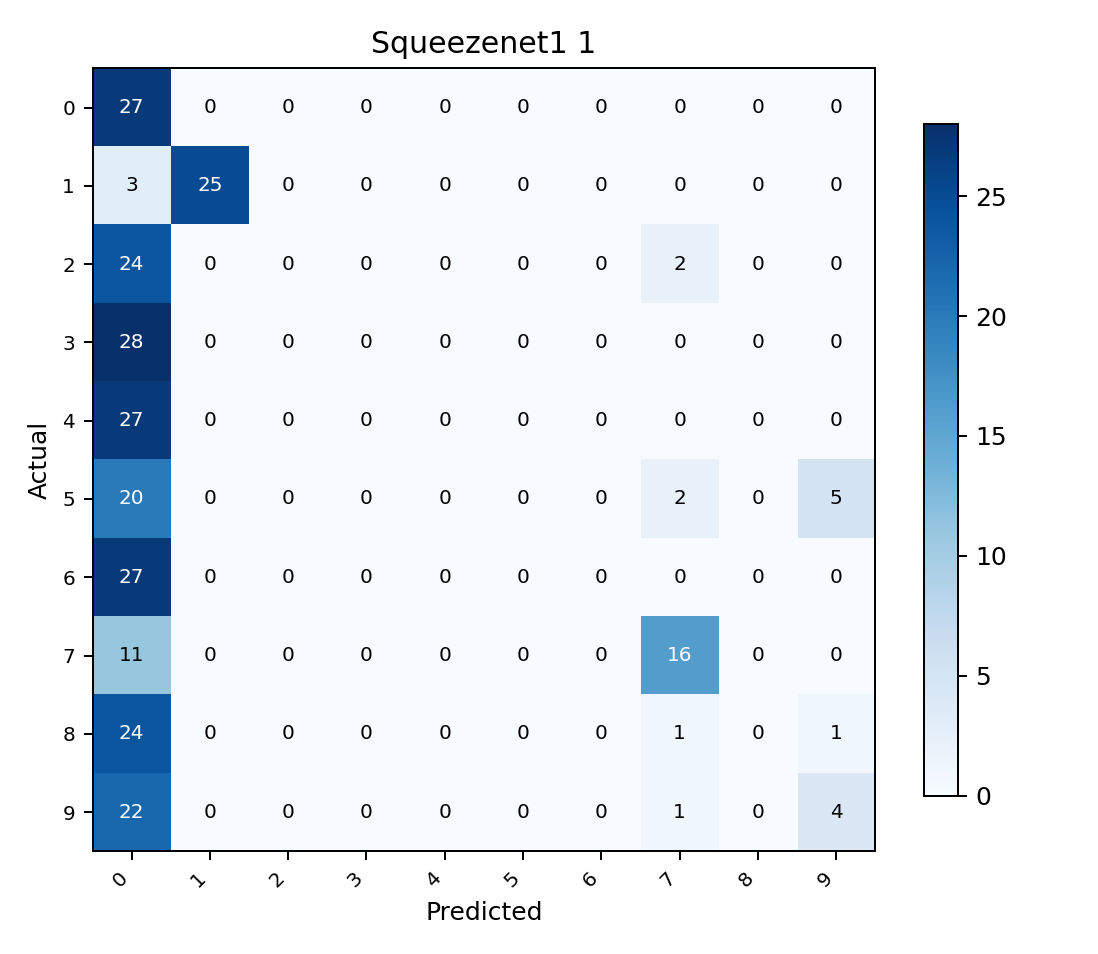
\includegraphics[width=0.46\linewidth]{../results/plots/squeezenet1_1_confusion.png}\caption{SqueezeNet1.1 training and validation loss (left) and test confusion matrix (right).}\end{figure}

Our transfer-learning implementation uses a frozen pretrained backbone and a replacement classifier head for seven epochs with Adam ($\eta=0.001$), followed by three epochs with a small portion of the final convolution layers unfrozen ($\eta=0.0001$). The pretrained backbone's batch-normalization running statistics were kept fixed. All networks use the same train/validation/test indices, but the custom models were trained on CPU and these two pretrained models on a Colab GPU, so their epoch times should not be compared as if they were obtained on the same hardware.

\section{Final trade-off discussion}
The Model B convolution operation replaces a full $3\times3$ convolution with a depthwise spatial step and a $1\times1$ channel-mixing step. This reduces both parameter memory and approximate multiplications. For edge devices, the best model is not always the one with the most accuracy; a smaller model may be easier to deploy when RAM, flash memory, and energy are limited.

Model B gave the highest efficiency and also the highest measured accuracy of the three small/edge-oriented models: 95.9\%, compared with MobileNetV2 (77.0\%) and SqueezeNet1.1 (26.7\%). ImageNet features learned from natural photos may transfer poorly to tiny, originally grayscale handwriting, even after classifier tuning. SqueezeNet particularly struggled on this setting, with several classes confused in its matrix. The pretrained models were trained for only ten epochs (seven classifier-head and three partial fine-tuning), while the custom networks ran for 25 epochs. Different schedules, pretrained initialization, and model capacity mean these results do not isolate the effect of architecture alone. The observed accuracies are dataset-specific rather than universal rankings. Their higher parameter counts and actual checkpoint sizes also make them harder to fit on very small devices. Neither on-device latency nor power consumption was measured.

The MAC counts here are analytical estimates for Conv2d and Linear operations only; actual deployment speed and memory depend on the inference library, memory access, processor features, quantization, and other overhead. We did not measure an embedded board. The digit images were already very small, so conclusions may not generalize to natural-color images. The evaluation uses one data split and one random seed. Repeating the tests with multiple seeds and a real edge board would make the conclusions stronger.

\section{Conclusion}
The depthwise-separable custom CNN meets the less-than-100,000 trainable parameter requirement with just 5,813 parameters. It achieves 95.9\% test accuracy on the recorded dataset using markedly fewer counted MACs than the standard CNN. Adam, SGD and momentum differ substantially in convergence at our fixed settings. In the completed transfer-learning trials, MobileNetV2 reached 77.0\% test accuracy and SqueezeNet1.1 reached 26.7\%, both below the custom networks on these low-resolution digits. Results depend on the dataset and training setup.

\paragraph{Code and reproducibility.} Full code, split indices and recorded metrics are provided with the submission. Repository: \url{https://github.com/Isira-Himal-Perera/CNN-for-Edge-Image-Classification}. Source results: \texttt{results/}.

\begin{thebibliography}{9}\small
\bibitem{assignment} S. K. Perera, ``EN3150 Assignment 03: Simple convolutional neural network to perform classification,'' University of Moratuwa, 2026.
\bibitem{digits} E. Alpaydin and C. Kaynak, ``Optical Recognition of Handwritten Digits,'' UCI Machine Learning Repository, \url{https://archive.ics.uci.edu/dataset/80/optical+recognition+of+handwritten+digits}.
\bibitem{sklearn} F. Pedregosa et al., ``Scikit-learn: Machine Learning in Python,'' Journal of Machine Learning Research, 2011.
\bibitem{beans} Makerere AI Lab, ``Beans leaf image dataset,'' \url{https://github.com/AI-Lab-Makerere/ibean}.
\bibitem{mobile} M. Sandler et al., ``MobileNetV2: Inverted Residuals and Linear Bottlenecks,'' CVPR, 2018.
\bibitem{squeeze} F. Iandola et al., ``SqueezeNet: AlexNet-level accuracy with 50x fewer parameters and $<$0.5MB model size,'' 2016.
\end{thebibliography}
\end{document}
